%
%----------------------------------------------------------------------------------------
%	PACKAGES AND DOCUMENT CONFIGURATIONS
%----------------------------------------------------------------------------------------
%
\documentclass[12pt]{article} %report, article, amsart, exam
\usepackage[letterpaper,margin=1in]{geometry}
\usepackage{fancyhdr,color}
\usepackage{tikz,graphicx,multicol}
\usepackage{amssymb,euscript,eufrak,nicefrac,enumitem}
\usepackage{amsfonts,amsmath,amsthm} %don't need with 'amsart' document class
\usepackage{hyperref}
\usepackage{comment}
\usepackage{scrextend} %needed for addmargin environment
\usepackage{graphicx} 
\usepackage{listings}
\usepackage{color}
\usepackage{accsupp}
\usepackage{booktabs}
\usepackage{subcaption}


\definecolor{dkblue}{rgb}{0,0,0.5}
\definecolor{comment}{rgb}{1,0,0}
\definecolor{mauve}{rgb}{.627,.126,.941}
\definecolor{purple}{rgb}{0.5, 0, 0.545098}


%
%----------------------------------------------------------------------------------------
%% Define headers & footers
%----------------------------------------------------------------------------------------

\pagestyle{fancy}
   \lhead{} 
   %\chead{Loyola University Chicago} 
   \rhead{}
   \renewcommand{\headrulewidth}{0pt}
   \addtolength{\footnotesep}{5mm}
%
%----------------------------------------------------------------------------------------
%% Some user-defined colors
%----------------------------------------------------------------
\setlength{\parskip}{1em}
\renewcommand{\baselinestretch}{1.3}
%
%----------------------------------------------------------------------------------------
%% BEGIN: topmatter
%----------------------------------------------------------------------------------------
%
\title{ COMP 464 - High Performance Computing \\ Stream2 Benchmark} % Title
\author{
Loyola University Chicago \\
Jose Luis Rodriguez 
} % Author name
\date{\today} % Date for the report
%
%% END: topmatter
%%------------------------------
\begin{document}
\maketitle
\thispagestyle{fancy}

%---------------------------------------------------------------------------------------- 
%	SECTION 1 - PROBLEM STATEMENT
%----------------------------------------------------------------------------------------

\section{Overview}
This report highlights the procedures and results of running the Stream2 C++ code that runs a series of experiments and generates a benchmark utilizing the Stampede2 supercomputer at The University of Texas at Austin's Texas Advanced Computing Center (TACC), the code is also execute on a Lenovo workstation running CentOS7 and Intel C++ library compilers, details and specifications to follow. 

The Stream2 benchmark runs a number of tests measuring the bandwidth of L1, L2, L3 cache, and main DRAM. The first benchmark uses GNU C++ compiler to build the Stream2 program on Stampede2 compute and login nodes as well as and the Lenovo workstation. After building the code with GNU or Intel compiler, the program is run and the output is recorded in the tables below. The specifications of each system are also recorded in the tables at the end of the report. The idea behind this experiment is to examine how the memory and cache behave during the different experience and to compare the Intel and GNU C++ compilers. 

%----------------------------------------------------------------------------------------
%	SECTION 2 - DESCRIPTION
%----------------------------------------------------------------------------------------

\section{Benchmark Analysis}

The stream2 code runs a number of loops over a sequence of experiments and various benchmarks:

\begin{table}[ht]
\centering
\resizebox{\textwidth}{!}{%
\begin{tabular}{cl}
\textbf{Benchmark} & \textbf{Description} \\ \midrule
FILL (MB/s) & Set all elements in an array to a particular value \\
COPY & Copy two arrays - one into the other \\
AXPY & Takes two arrays make changes and writes back (Alpha x plus y) \\
DOT & Sum of the product of two arrays (Dot Product) \\ \bottomrule
\end{tabular}%
}
\end{table}

The benchmarks above were run on Stampede2 following two approaches. The first the code runs on the compute Node by requesting a flat quadrant and executing the code on that node. The second approach uses the $numactl$ command to run the code using the MCDRAM on the computer node. 

The benchmarks were run with a min array size of 30 Bytes and three different max array sizes (20Mb, 25Mb, and 30Mb).This report only highlights the results when using the largest array size (30Mb) as the goal is to stress the last level cache and setting the number of tests between the min and max array size to 50. The same parameters were used for all benchmarks, compilers and nodes. To calculate the size of the array at the $n$ iteration the following metric was used:

\begin{table}[ht]
\resizebox{\textwidth}{!}{%
\begin{tabular}{cc}
\textbf{Benchmark} & \textbf{Array Size (Metric) } \\  \midrule
FILL  & $(\text{n\_iteration})(8 \text{ bytes/double})(1 \text{ double/iteration})$ \\
COPY & $(\text{n\_iteration})(8 \text{ bytes/double})(2 \text{ double/iteration})$ \\
AXPY & $(\text{n\_iteration})(8 \text{ bytes/double})(3 \text{ double/iteration})$ \\
DOT & $(\text{n\_iteration})(8 \text{ bytes/double})(2 \text{ double/iteration})$ \\ \bottomrule
\end{tabular}%
}
\end{table}

\newpage

\subsection{Benchmark Results}

In Figure.1 Stampede2 compute node using the GNU compiler, we can see how the benchmark that uses most bandwidth is the \textsc{COPY} benchmark, with a top performance at $26kb$ right before filling the $32kb$ L1 cache then we see another drop at approximately after 534kb array size when L2 cache gets  filled. The other benchmarks seem to behave more or less similarly, some of them show some drops but nothing close to what the \textsc{COPY} benchmark experience.


\begin{figure}[htb]
\caption{Stampede2 Compute Node - GNU Compiler}\label{fig:benchmark01}
\centering
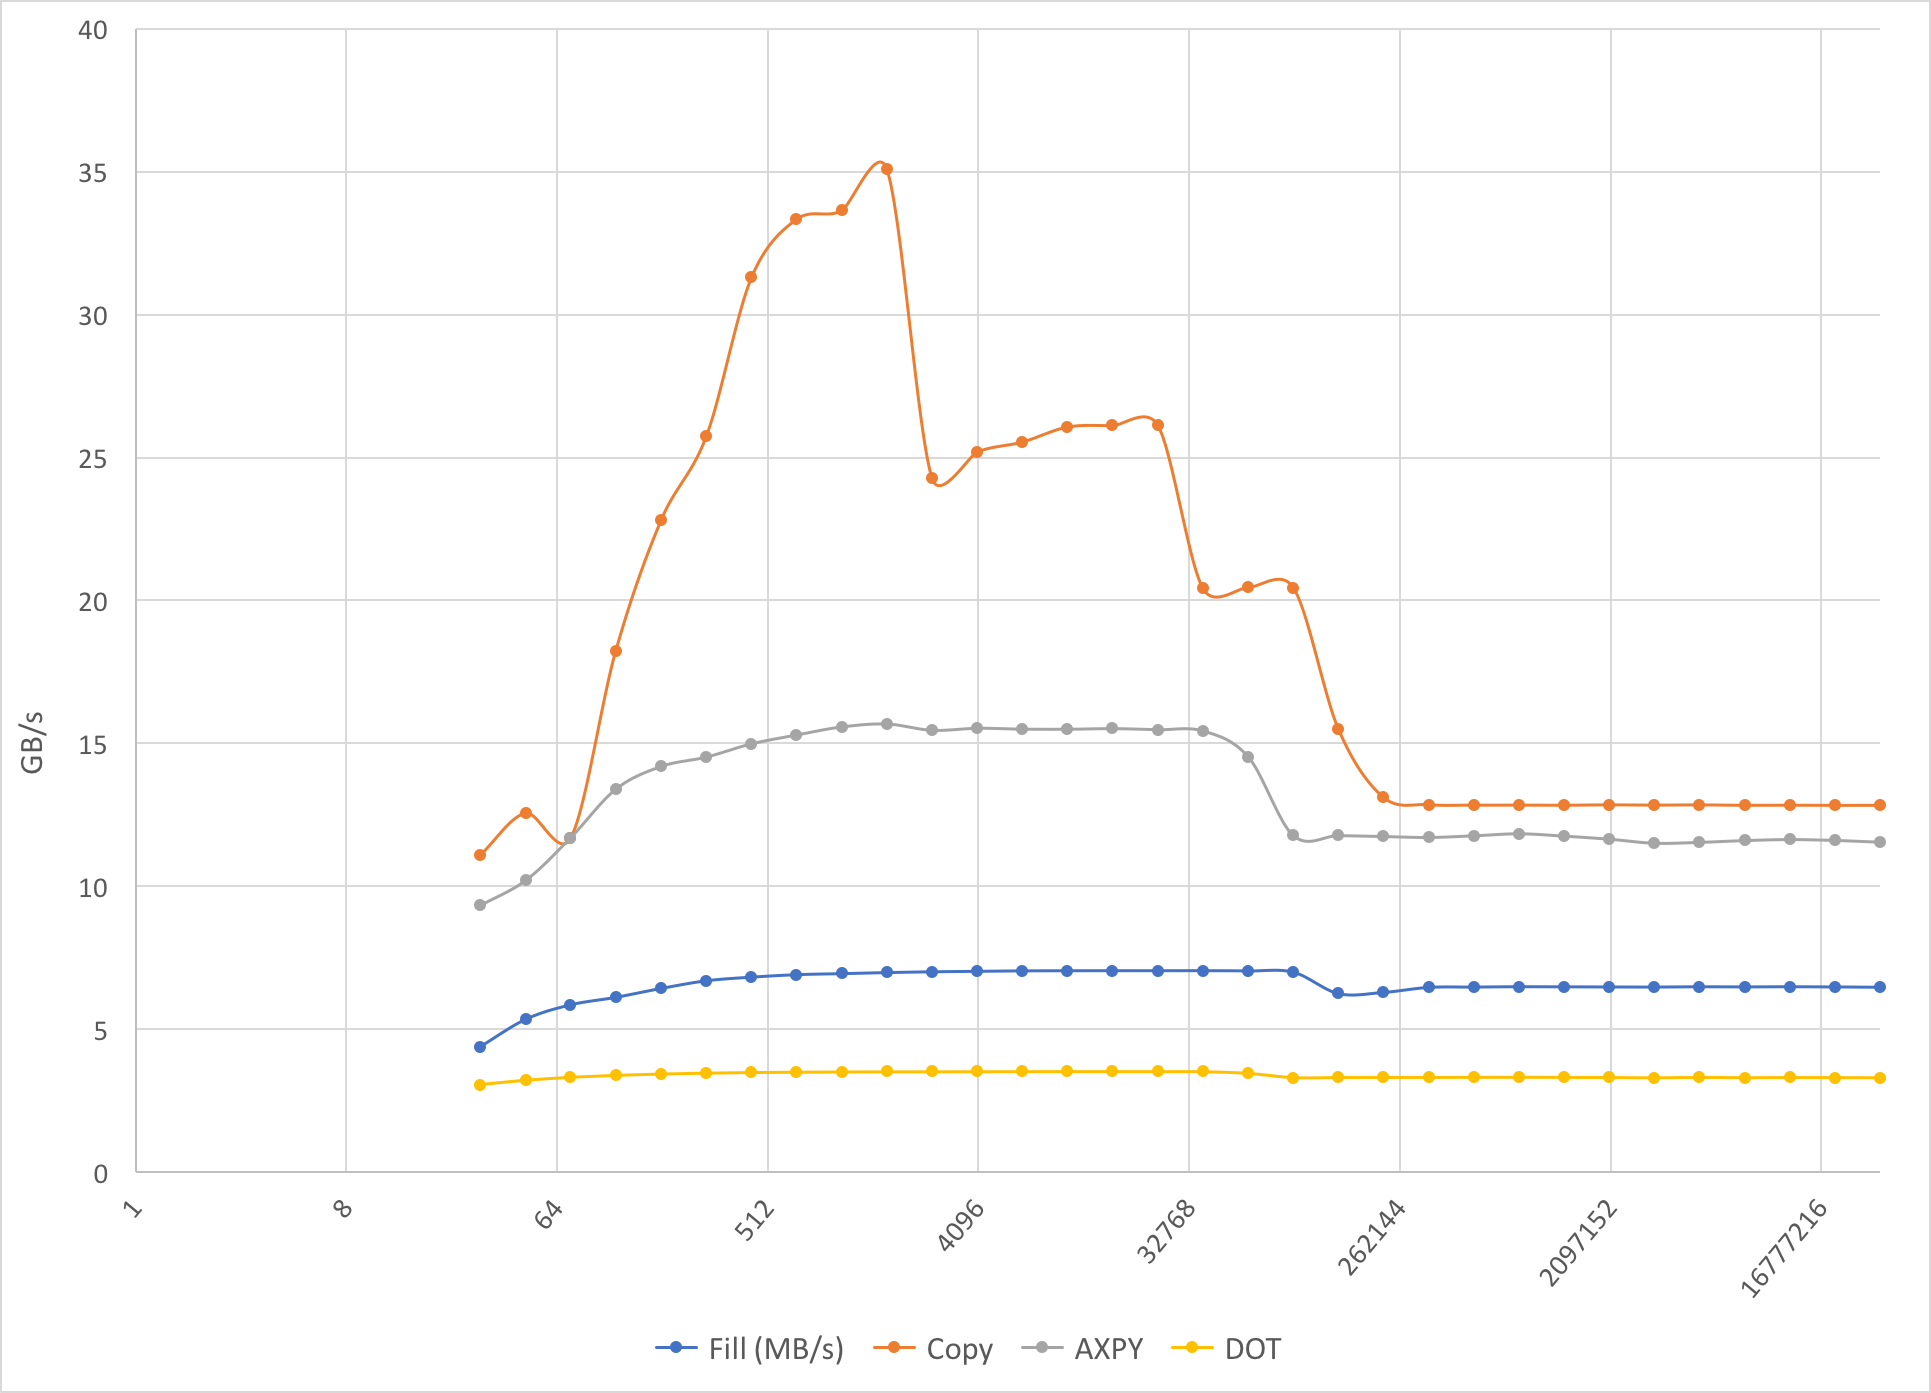
\includegraphics[width=\textwidth,keepaspectratio]{imgs/img01.png}
\end{figure} 

\newpage

Now in Figure.2 we change the compiler to Intel's C++ compiler and we can see significant changes on all the benchmarks. The most prominent change from the previous figure is the \textsc{AXPY}  benchmark that peeks approximately around $40kb$ with a much higher bandwidth almost 120 times higher compared with the GNU compiler.  The \textsc{FILL} benchmark also shows signs of a significant drop with a peek at 32kb and $100$Gb\/s to $40$Gb\/s  after the $L1$ gets filled.

\begin{figure}[htb]
\caption{Stampede2 Compute Node - Intel Compiler}\label{fig:benchmark02}
\centering
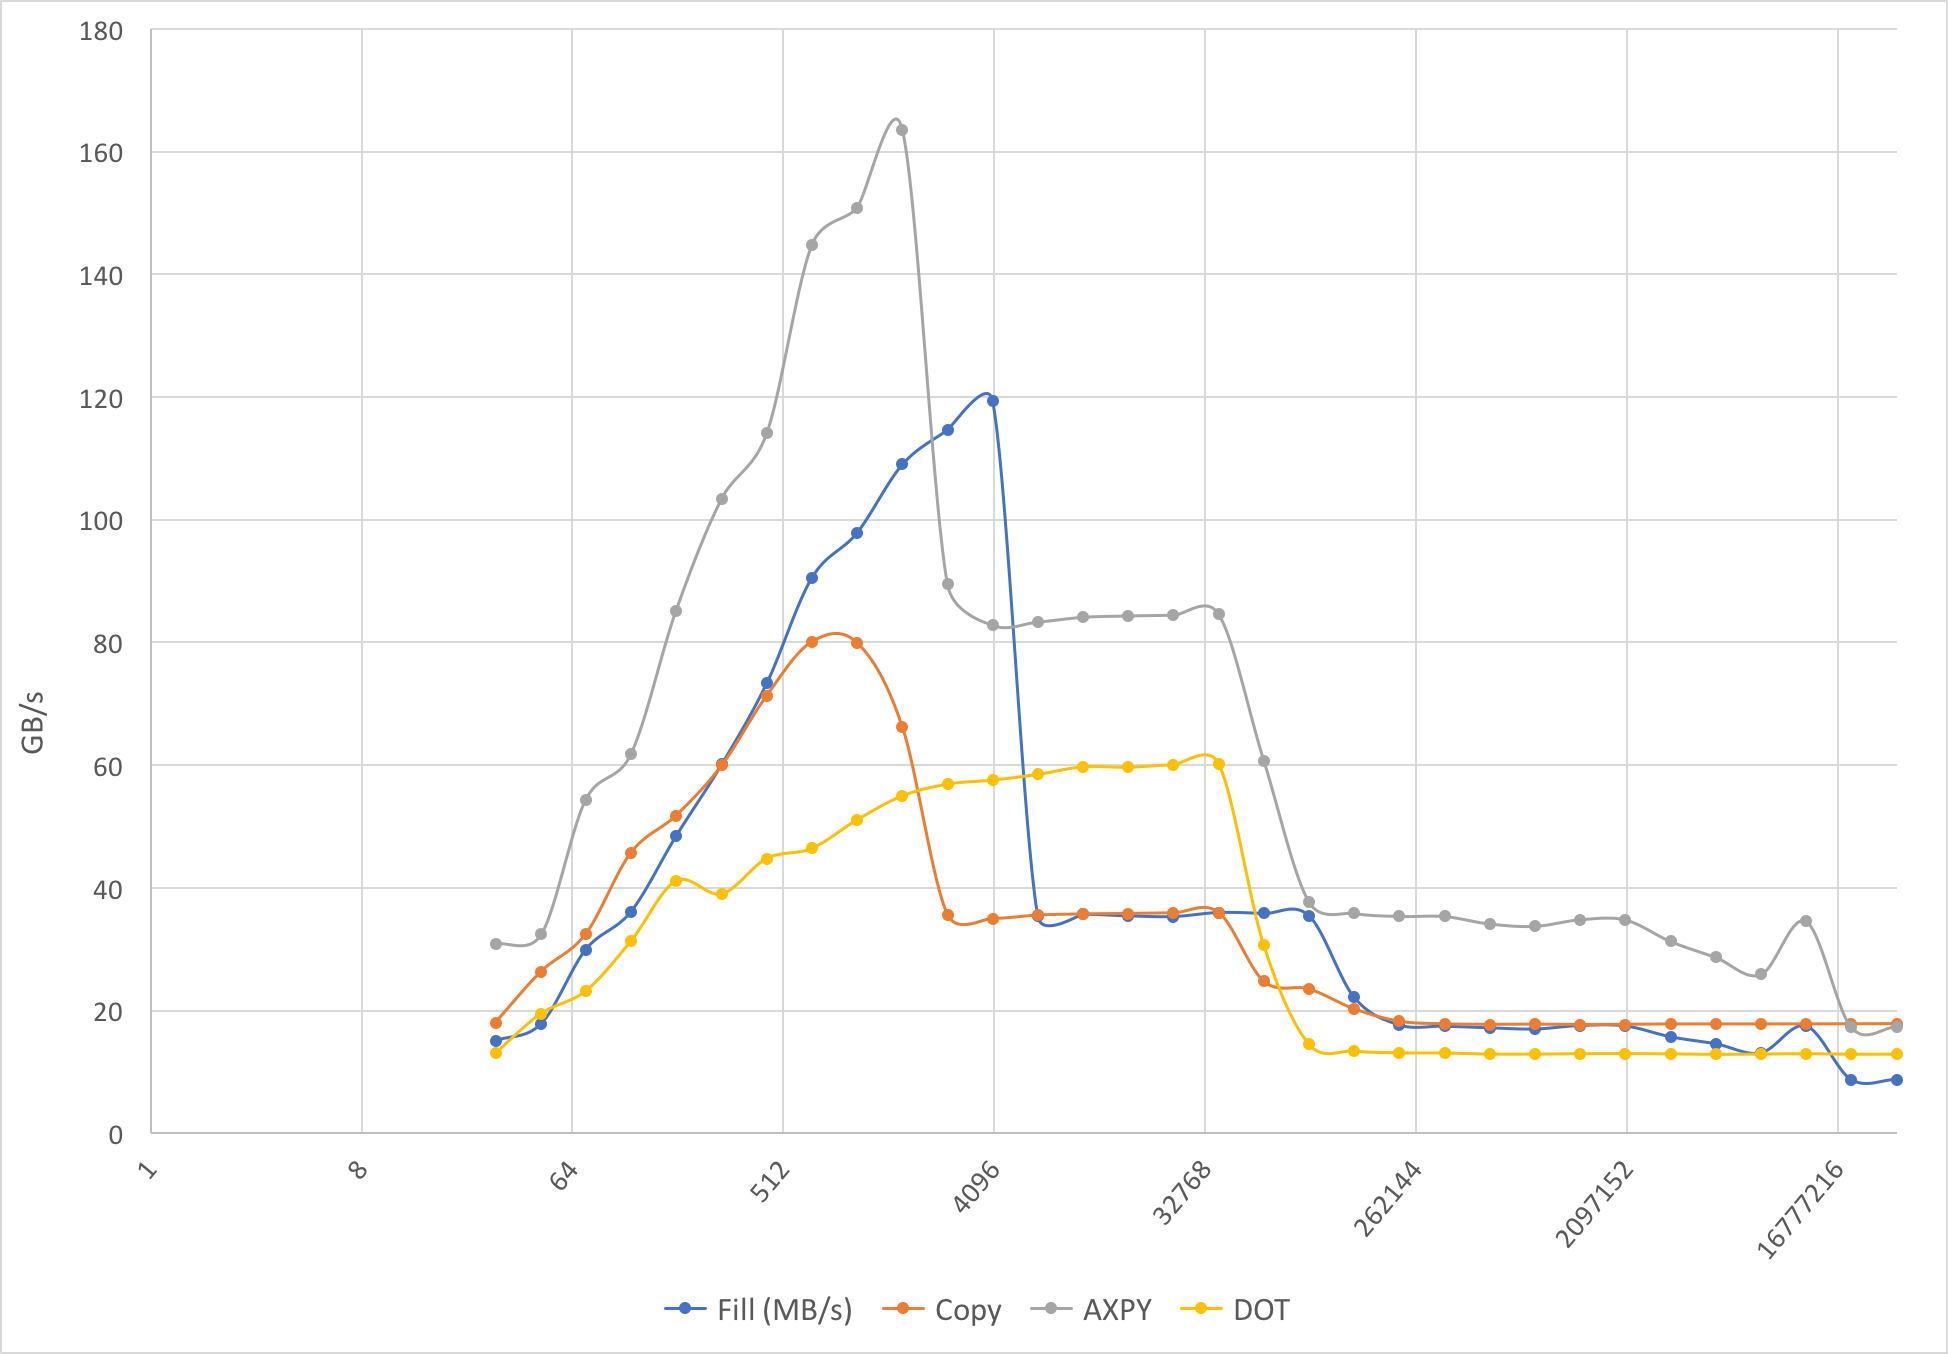
\includegraphics[width=\textwidth,keepaspectratio]{imgs/img02.png}
\end{figure}

\newpage

Figure.3 was generated using the \verb|numactl| command on the compute node that allows to use a much faster memory  (MCDRAM), this benchmark also uses the Intel library. The bandwidth increase almost twice compared with the previous benchmark but there is a more drastic drop of performance when the L1 cache is filled. We can see how when the array size is large enough almost all benchmarks behave similarly as they are accessing memory directly, here is the command use to run the benchmark: \\ \verb| numactl --membind=1 --cpunodebind=0 ./stream2 -max 30000000|

\begin{figure}[htb]
\caption{Stampede2 Compute Node - Intel Compiler}\label{fig:benchmark03}
\centering
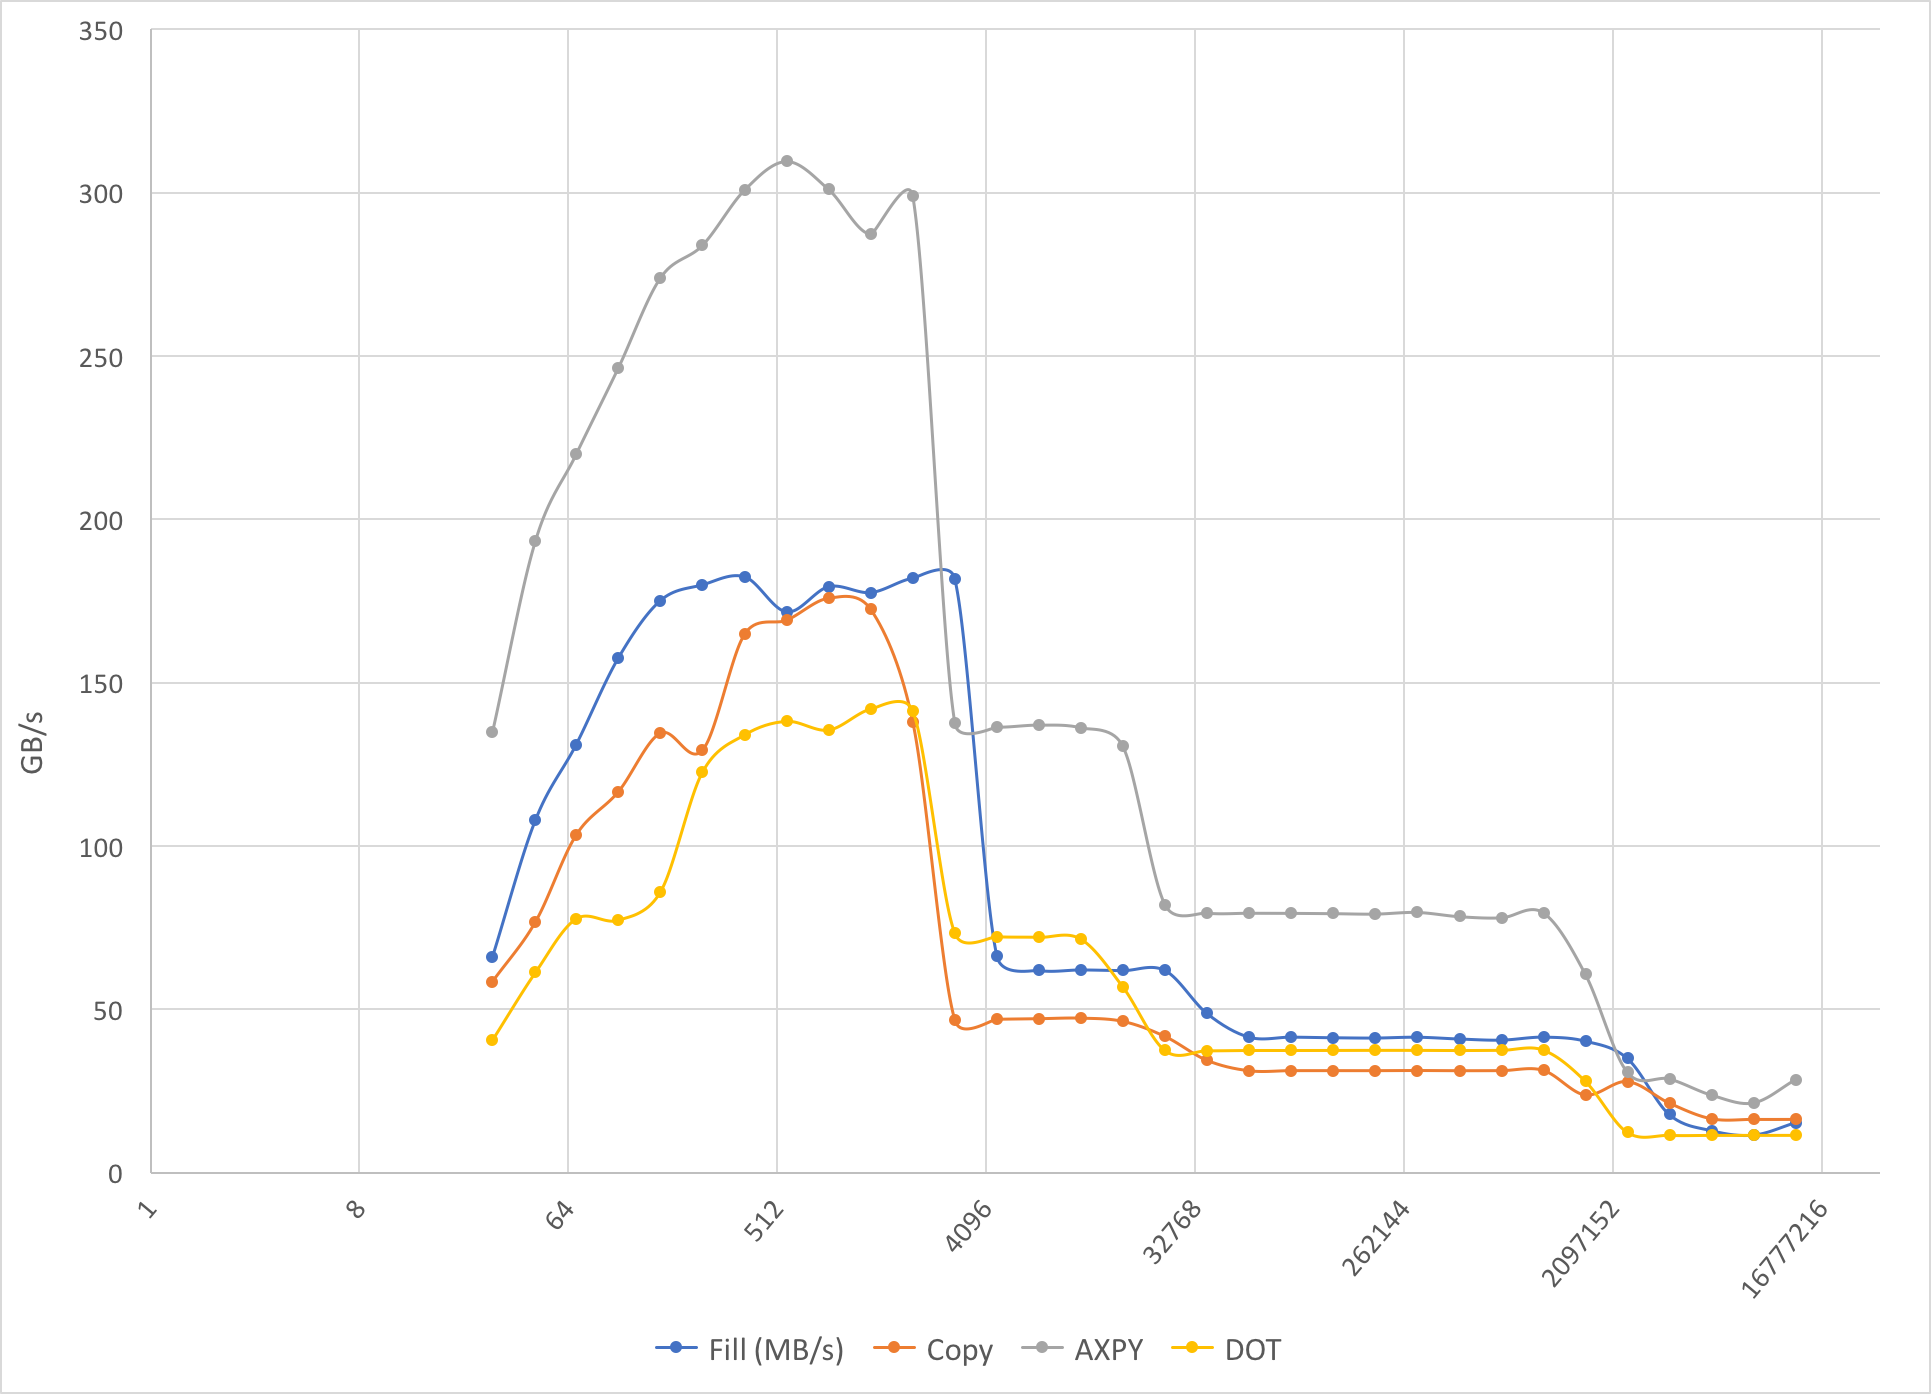
\includegraphics[width=\textwidth,keepaspectratio]{imgs/img03.png}
\end{figure}

\newpage

Figure.4 was generated using a Lenovo Workstation, the bandwidth is almost $1/3$ compared with the Stampede2 compute node, we can see similar drops when the array size filled L1 cache, L2 cache an then access memory directly is interesting to see how the different benchmarks plateau in each cached level and they become flat at the when the array size is large enough.

\begin{figure}[htb]
\caption{Lenovo Workstation - Intel Compiler}\label{fig:benchmark04}
\centering
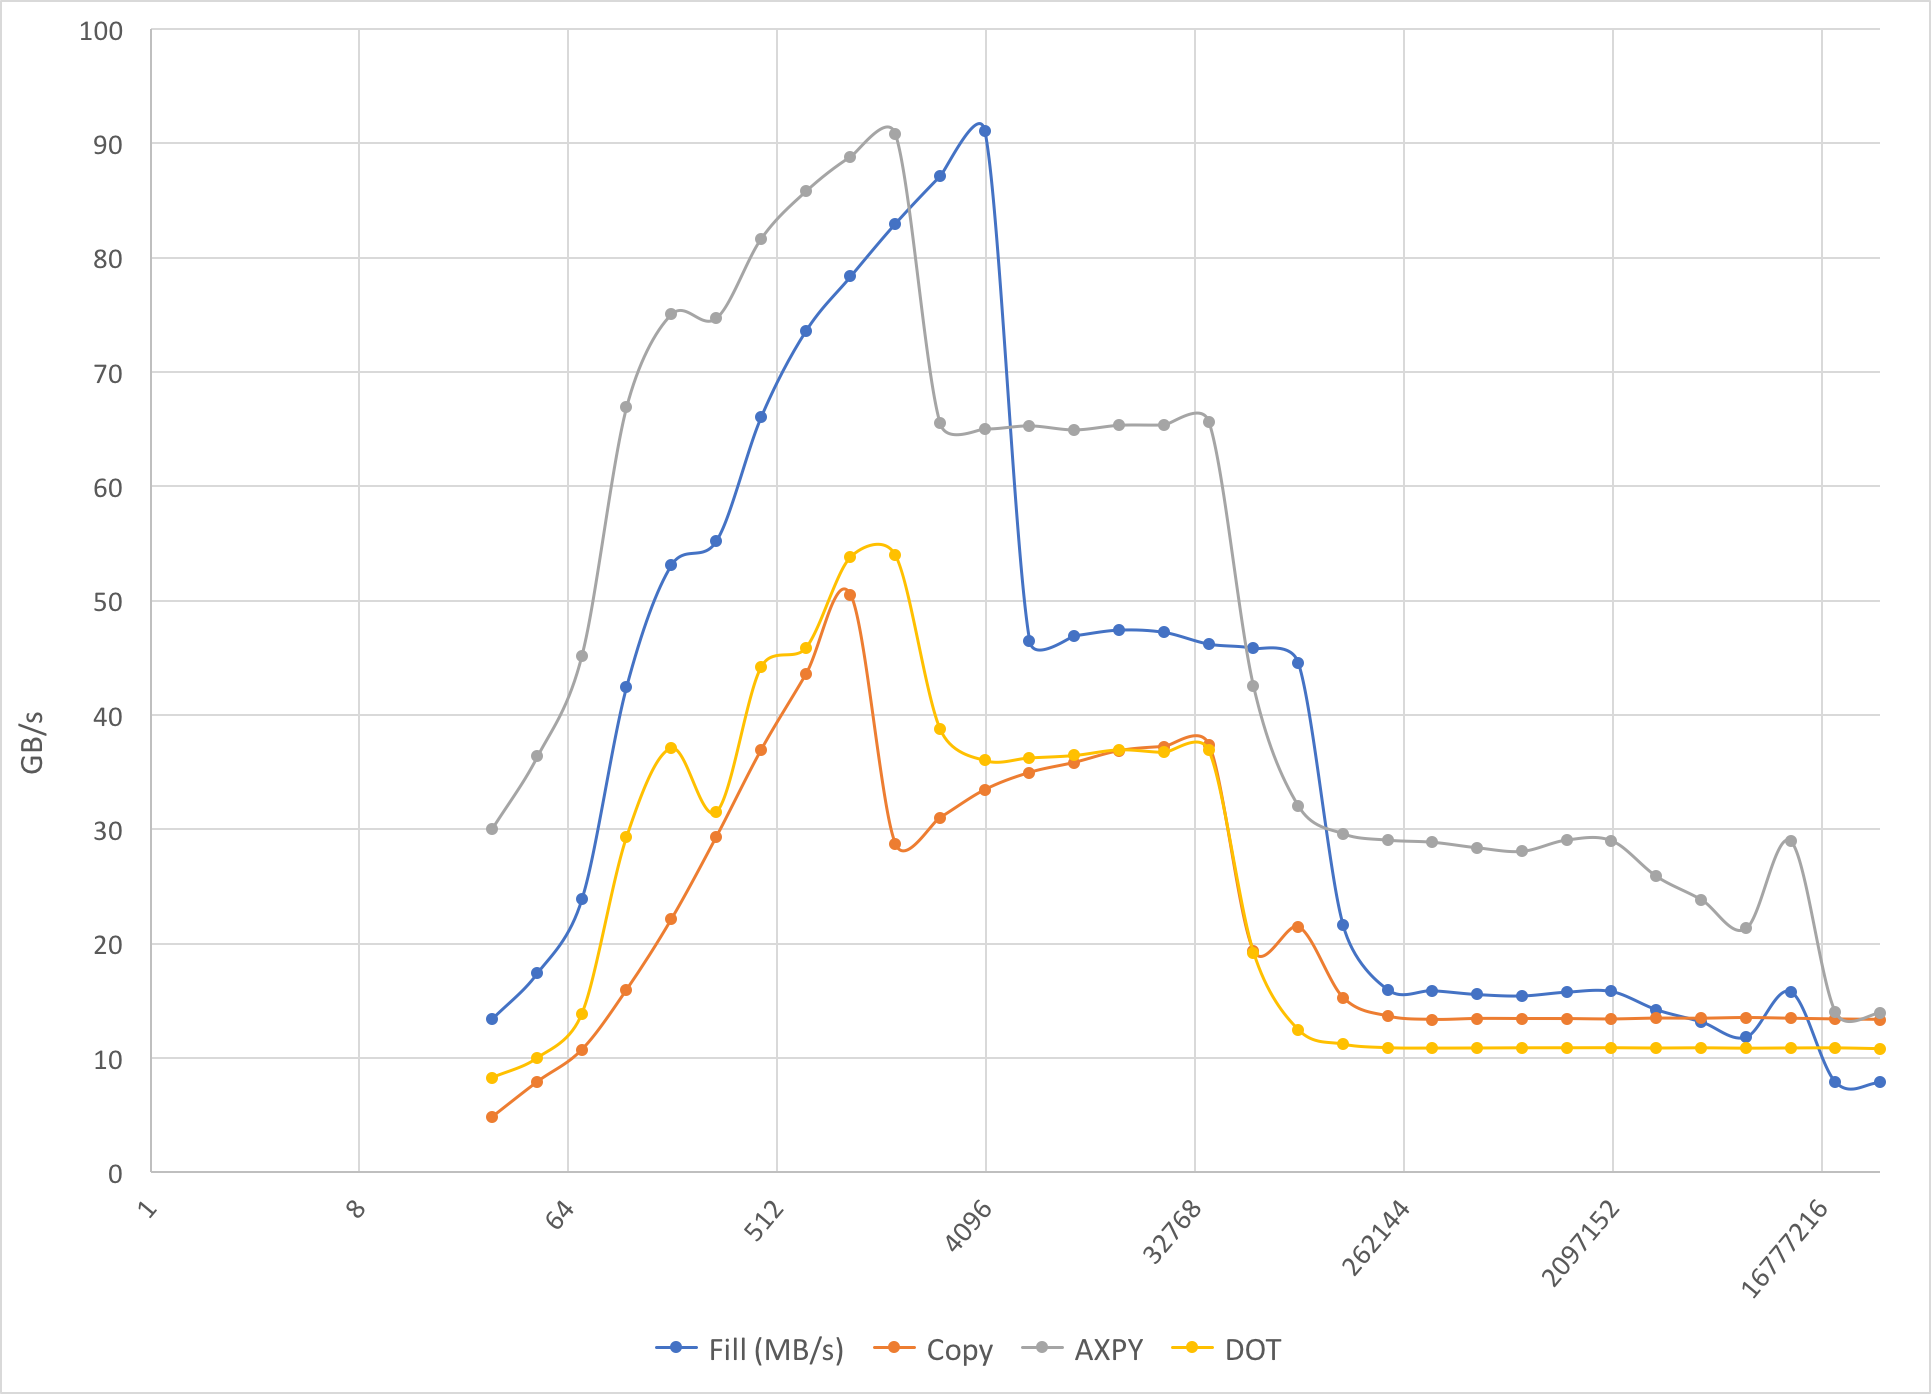
\includegraphics[width=\textwidth,keepaspectratio]{imgs/img04.png}
\end{figure}

\newpage

The last chart was generated by running the same \verb|numactl| command on the Stampede2 login node instate of the compute node. It is interesting to see how in this case the bandwidth plateau earlier and stay there for a couple of cycles before it drops again simnifically, when compared with the compute node the bandwidth are very similar.  

\begin{figure}[htb]
\caption{Stampede2 Login Node - Intel Compiler}\label{fig:benchmark05}
\centering
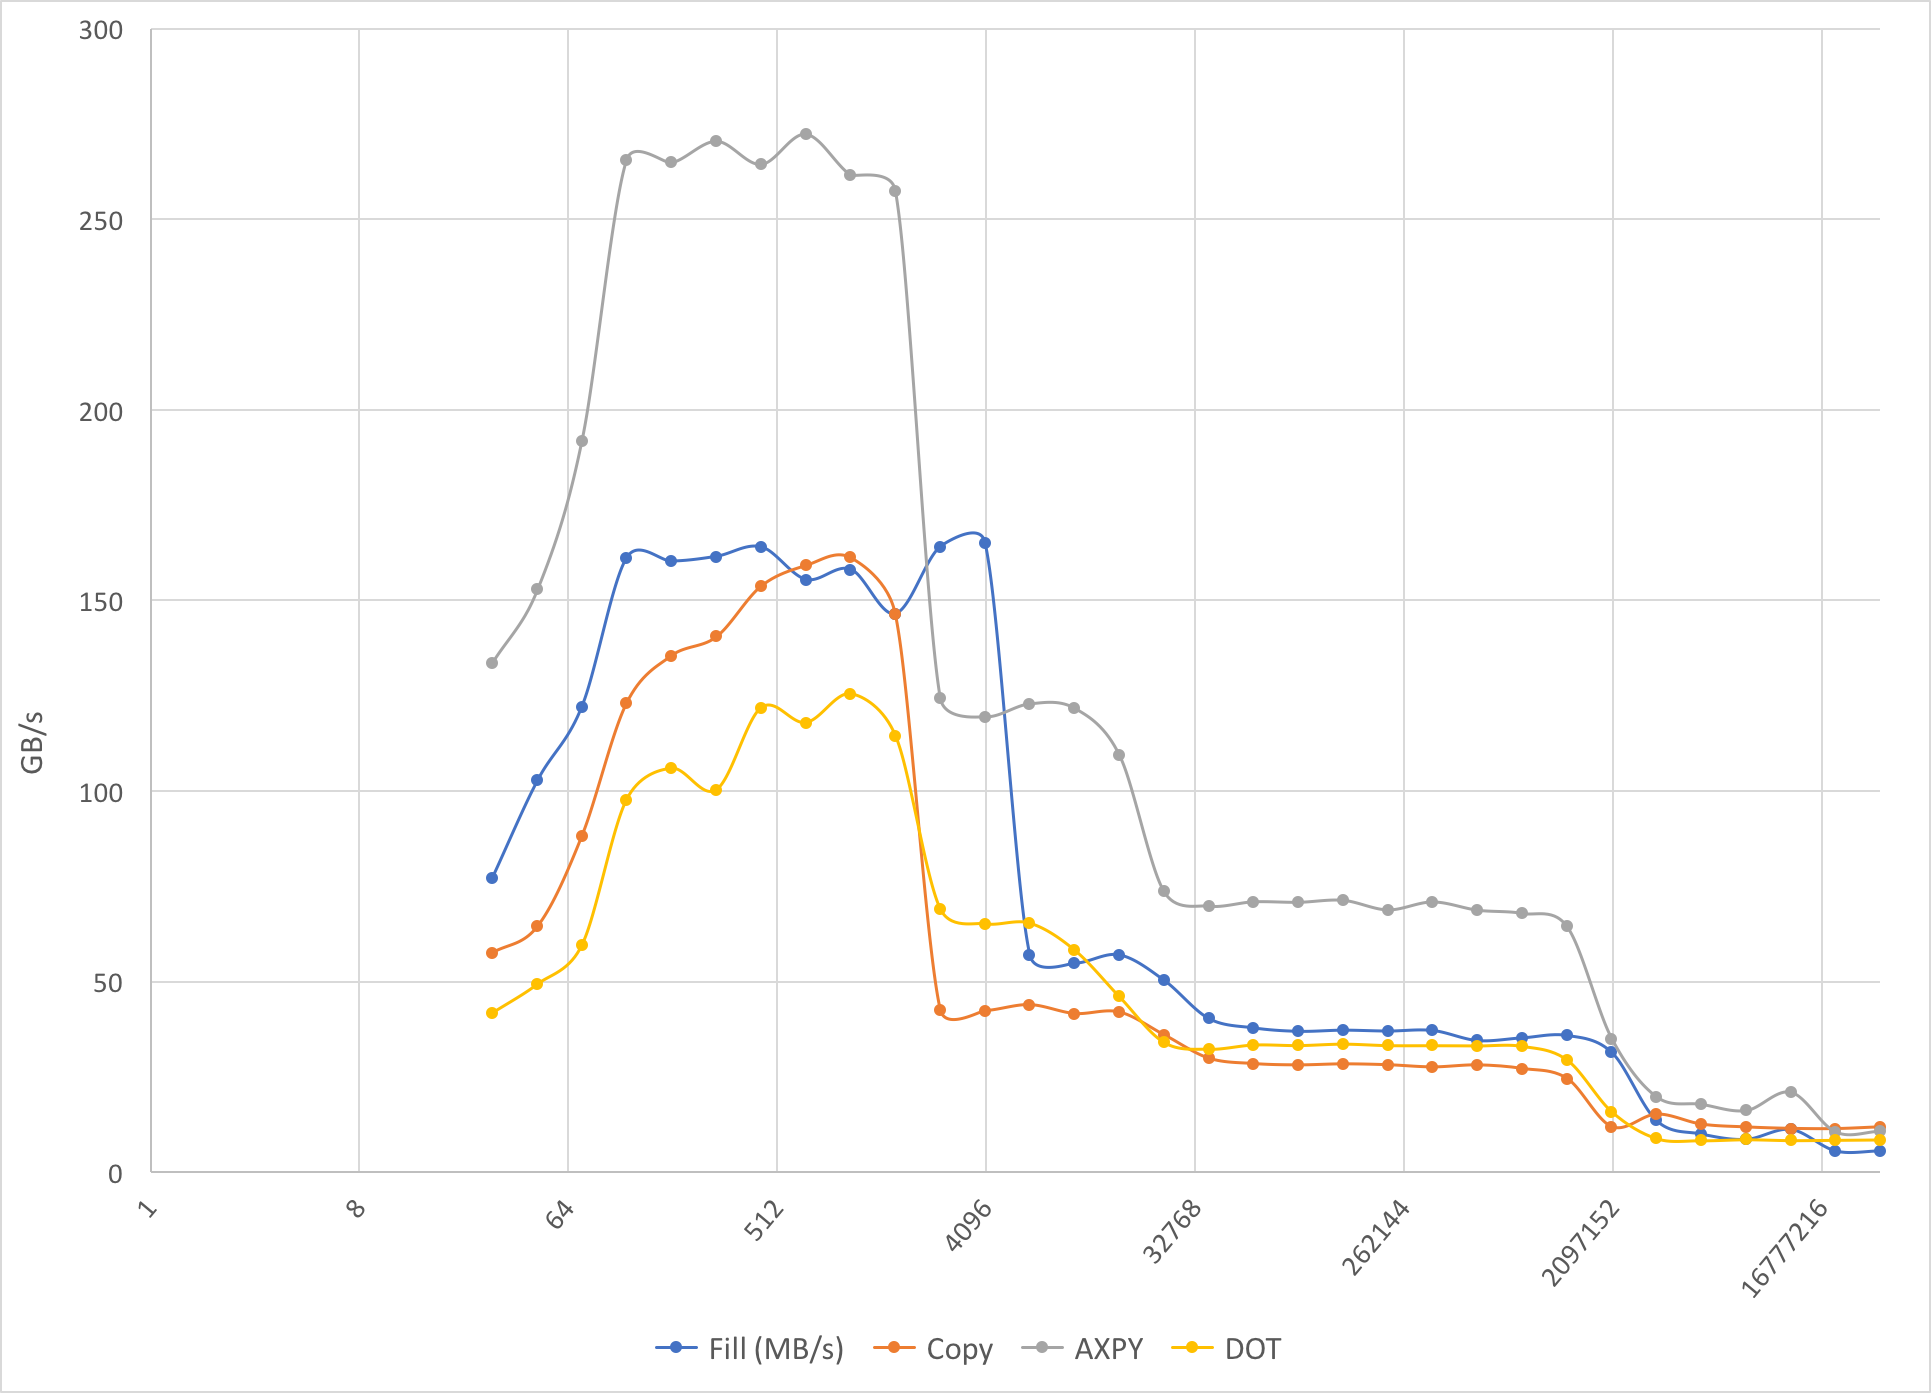
\includegraphics[width=\textwidth,keepaspectratio]{imgs/img05.png}
\end{figure}

\newpage


%----------------------------------------------------------------
%	SECTION 3 - REFERENCE
%----------------------------------------------------------------

\section{Reference}

\begin{flushleft}
Stampede2 User Guide -- Managing Memory \\ \url{https://portal.tacc.utexas.edu/user-guides/stampede2#managingmemory}

Introduction to High Performance Scientific Computing -- Victor Eijkhout \\ \url{http://pages.tacc.utexas.edu/~eijkhout/istc/istc.html}

\end{flushleft}


\begin{table}[]
\centering
\caption{Stampede2 - Compute Node (knl) - System Information}
\resizebox{\textwidth}{!}{%
\begin{tabular}{@{}ll@{}}
\toprule
\textbf{Architecture} & x86\_64 \\ \midrule
\textbf{CPU op-mode(s)} & 32-bit, 64-bit \\
\textbf{Byte Order} & Little Endian \\
\textbf{CPU(s)} & 272 \\
\textbf{On-line CPU(s) list} & 0-271 \\
\textbf{Thread(s) per core} & 4 \\
\textbf{Core(s) per socket} & 68 \\
\textbf{Socket(s)} & 1 \\
\textbf{NUMA node(s)} & 2 \\
\textbf{Vendor ID} & GenuineIntel \\
\textbf{CPU family} & 6 \\
\textbf{Model} & 87 \\
\textbf{Model name} & Intel(R) Xeon Phi(TM) CPU 7250 @ 1.40GHz \\
\textbf{Stepping} & 1 \\
\textbf{CPU MHz} & 1255.132 \\
\textbf{BogoMIPS} & 2793.44 \\
\textbf{L1d cache} & 32K \\
\textbf{L1i cache} & 32K \\
\textbf{L2 cache} & 1024K \\
\textbf{NUMA node0 CPU(s)} & 0-271 \\
\textbf{NUMA node1 CPU(s)} &  \\ \bottomrule
\end{tabular}%
}
\end{table}



\begin{table}[]
\centering
\caption{Lenovo Workstation - CentOS7 - System Information}
\resizebox{\textwidth}{!}{%
\begin{tabular}{@{}ll@{}}
\toprule
\textbf{Architecture} & x86\_64 \\ \midrule
\textbf{CPU op-mode(s)} & 32-bit, 64-bit \\
\textbf{Byte Order} & Little Endian \\
\textbf{CPU(s)} & 40 \\
\textbf{On-line CPU(s) list} & 0-39 \\
\textbf{Thread(s) per core} & 2 \\
\textbf{Core(s) per socket} & 10 \\
\textbf{Socket(s)} & 2 \\
\textbf{NUMA node(s)} & 2 \\
\textbf{Vendor ID} & GenuineIntel \\
\textbf{CPU family} & 6 \\
\textbf{Model} & 79 \\
\textbf{Model name} & Intel(R) Xeon(R) CPU E5-2630 v4 @ 2.20GHz \\
\textbf{Stepping} & 1 \\
\textbf{CPU MHz} & 1291.382 \\
\textbf{CPU max MHz} & 3100.0000 \\
\textbf{CPU min MHz} & 1200.0000 \\
\textbf{BogoMIPS} & 4389.67 \\
\textbf{Virtualization} & VT-x \\
\textbf{Hypervisor vendor} & vertical \\
\textbf{Virtualization type} & full \\
\textbf{L1d cache} & 32K \\
\textbf{L1i cache} & 32K \\
\textbf{L2 cache} & 256K \\
\textbf{L3 cache} & 25600K \\
\textbf{NUMA node0 CPU(s)} & 0-9,20-29 \\
\textbf{NUMA node1 CPU(s)} & 10-19,30-39 \\ \bottomrule
\end{tabular}%
}
\end{table}


\begin{table}[]
\centering
\caption{Stampede2 Compute Node - GNU Compiler}
\resizebox{\textwidth}{!}{%
\begin{tabular}{@{}llllll@{}}
\toprule
\textbf{Size (iterations)} & \textbf{Fill (MB/s)} & \textbf{Copy} & \textbf{AXPY} & \textbf{DOT} & \textbf{Uncertainty (\%)} \\ \midrule
30 & 4393.162231 & 11104.6881 & 9336.596419 & 3051.421911 & 1.90\% \\
47 & 5350.378441 & 12565.39118 & 10220.65398 & 3209.223289 & 1.50\% \\
73 & 5853.695055 & 11687.71559 & 11702.86902 & 3316.590107 & 1.10\% \\
114 & 6116.984412 & 18242.91233 & 13398.08149 & 3388.55338 & 0.70\% \\
178 & 6427.522021 & 22800.19441 & 14194.47704 & 3438.065904 & 0.50\% \\
279 & 6698.122428 & 25768.72093 & 14527.06717 & 3472.020319 & 0.30\% \\
435 & 6824.597812 & 31305.48923 & 14986.95631 & 3493.9909 & 0.20\% \\
679 & 6911.333146 & 33345.25901 & 15297.0655 & 3507.619116 & 0.10\% \\
1060 & 6948.028771 & 33650.79479 & 15578.51236 & 3515.477478 & 0.10\% \\
1656 & 6985.001187 & 35089.74094 & 15680.55274 & 3520.668913 & 0.10\% \\
2586 & 7012.81148 & 24271.79651 & 15462.08087 & 3521.383827 & 0.00\% \\
4038 & 7029.597848 & 25202.06851 & 15531.84052 & 3525.104143 & 0.00\% \\
6305 & 7044.938436 & 25549.57693 & 15502.22589 & 3527.599249 & 0.00\% \\
9846 & 7050.075265 & 26072.88131 & 15498.96218 & 3529.112917 & 0.00\% \\
15374 & 7051.78082 & 26124.29129 & 15519.55808 & 3528.904854 & 0.00\% \\
24008 & 7050.994641 & 26121.05296 & 15482.61471 & 3527.958451 & 0.00\% \\
37488 & 7051.782966 & 20421.04818 & 15437.97559 & 3523.761178 & 0.00\% \\
58539 & 7042.233872 & 20459.72158 & 14530.19158 & 3463.650355 & 0.00\% \\
91410 & 6996.433371 & 20445.17519 & 11782.12811 & 3306.784882 & 0.00\% \\
142738 & 6248.110944 & 15491.29423 & 11778.74414 & 3309.431658 & 0.00\% \\
222889 & 6290.558991 & 13109.06205 & 11746.50454 & 3311.366333 & 0.00\% \\
348047 & 6464.796754 & 12858.42716 & 11715.18304 & 3313.983805 & 0.00\% \\
543483 & 6477.457041 & 12841.93352 & 11772.74996 & 3316.270979 & 0.00\% \\
848661 & 6489.448093 & 12842.14791 & 11843.17557 & 3319.445295 & 0.00\% \\
1325203 & 6485.506785 & 12838.69628 & 11761.03164 & 3314.821514 & 0.00\% \\
2069336 & 6480.942411 & 12851.09811 & 11653.18953 & 3309.260037 & 0.00\% \\
3231315 & 6477.659875 & 12842.6458 & 11513.15796 & 3300.587295 & 0.00\% \\
5045773 & 6487.756168 & 12849.37284 & 11543.48494 & 3313.220334 & 0.00\% \\
7879091 & 6483.470428 & 12836.38542 & 11605.7627 & 3304.53413 & 0.00\% \\
12303381 & 6488.676065 & 12838.86536 & 11641.5715 & 3308.75048 & 0.00\% \\
19212013 & 6481.651785 & 12834.44793 & 11610.01186 & 3306.78088 & 0.00\% \\
30000000 & 6470.497548 & 12835.64937 & 11548.34264 & 3302.602269 & 0.00\% \\ \bottomrule
\end{tabular}%
}
\end{table}

\begin{table}[]
\centering
\caption{Stampede2 Compute Node - Intel Compiler}
\resizebox{\textwidth}{!}{%
\begin{tabular}{@{}llllll@{}}
\toprule
\textbf{Size (iterations)} & \textbf{Fill (MB/s)} & \textbf{Copy} & \textbf{AXPY} & \textbf{DOT} & \textbf{Uncertainty (\%)} \\ \midrule
30 & 15076.32499 & 18053.85978 & 30906.00129 & 13095.05445 & 6.60\% \\
47 & 17845.85505 & 26331.5801 & 32417.78294 & 19488.76166 & 5.00\% \\
73 & 29924.64285 & 32466.36848 & 54363.37106 & 23197.67158 & 5.40\% \\
114 & 36117.31918 & 45700.79007 & 61812.05105 & 31316.48663 & 4.20\% \\
178 & 48447.62984 & 51785.3116 & 85184.33885 & 41119.4245 & 3.60\% \\
279 & 60122.11714 & 59952.00819 & 103393.6844 & 39016.32316 & 2.80\% \\
435 & 73345.94715 & 71328.83551 & 114061.8083 & 44778.14129 & 2.20\% \\
679 & 90559.47399 & 80118.81023 & 144701.2393 & 46433.42544 & 1.70\% \\
1060 & 97900.40832 & 79957.29085 & 150806.9369 & 51074.56497 & 1.20\% \\
1656 & 109010.6951 & 66252.65334 & 163545.0942 & 54977.686 & 0.90\% \\
2586 & 114663.1208 & 35637.41072 & 89477.22895 & 56897.35007 & 0.60\% \\
4038 & 119417.9424 & 34996.98606 & 82780.89141 & 57565.11103 & 0.40\% \\
6305 & 35355.22437 & 35523.42247 & 83304.1754 & 58488.79063 & 0.10\% \\
9846 & 35690.26359 & 35714.49021 & 84088.76572 & 59724.16582 & 0.00\% \\
15374 & 35436.22662 & 35793.96904 & 84307.55835 & 59648.55565 & 0.00\% \\
24008 & 35322.30819 & 35900.19821 & 84432.10233 & 60073.95713 & 0.00\% \\
37488 & 35981.74332 & 35955.22864 & 84592.11752 & 60231.84392 & 0.00\% \\
58539 & 35828.34256 & 24737.90178 & 60757.13892 & 30640.1173 & 0.00\% \\
91410 & 35446.20978 & 23479.55979 & 37724.09292 & 14512.03045 & 0.00\% \\
142738 & 22159.83159 & 20235.74442 & 35858.4413 & 13378.82375 & 0.00\% \\
222889 & 17643.34403 & 18218.83898 & 35368.76334 & 13088.50196 & 0.00\% \\
348047 & 17438.23319 & 17792.17854 & 35354.06848 & 13054.44029 & 0.00\% \\
543483 & 17176.52069 & 17709.30278 & 34143.76344 & 12884.22877 & 0.00\% \\
848661 & 16982.16663 & 17734.60235 & 33759.5537 & 12884.06601 & 0.00\% \\
1325203 & 17554.79988 & 17680.34222 & 34829.10835 & 12947.07033 & 0.00\% \\
2069336 & 17483.75813 & 17706.67857 & 34799.37236 & 12972.67719 & 0.00\% \\
3231315 & 15715.29774 & 17768.26712 & 31289.79077 & 12922.9988 & 0.00\% \\
5045773 & 14569.38395 & 17767.62359 & 28677.94044 & 12841.36212 & 0.00\% \\
7879091 & 13100.15665 & 17772.13825 & 25901.08037 & 12891.50194 & 0.00\% \\
12303381 & 17474.37463 & 17779.8349 & 34532.61176 & 12941.04067 & 0.00\% \\
19212013 & 8732.041736 & 17793.79032 & 17318.09854 & 12866.99193 & 0.00\% \\
30000000 & 8762.057034 & 17817.95605 & 17392.93009 & 12871.03108 & 0.00\% \\ \bottomrule
\end{tabular}%
}
\end{table}

%----------------------------------------------------------------------------------------

\begin{table}[]
\centering
\caption{Lenovo Workstation - CentOS7 - Intel Compiler}
\resizebox{\textwidth}{!}{%
\begin{tabular}{@{}llllll@{}}
\toprule
\textbf{Size (iterations)} & \textbf{Fill (MB/s)} & \textbf{Copy} & \textbf{AXPY} & \textbf{DOT} & \textbf{Uncertainty (\%)} \\ \midrule
30 & 66112.72533 & 58494.27656 & 134909.179 & 40619.71983 & 28.90\% \\
46 & 107910.7797 & 76766.52557 & 193409.6647 & 61297.77476 & 30.70\% \\
69 & 131018.6842 & 103335.0823 & 219953.1734 & 77714.30418 & 24.90\% \\
105 & 157502.2839 & 116613.9987 & 246384.2462 & 77300.33301 & 19.70\% \\
160 & 175129.5372 & 134572.54 & 274035.1305 & 86039.6104 & 14.30\% \\
243 & 179923.0444 & 129394.9134 & 284017.764 & 122605.4301 & 9.70\% \\
370 & 182336.1625 & 164909.6116 & 300930.7027 & 134019.6058 & 6.50\% \\
562 & 171646.9864 & 169175.5295 & 309648.0482 & 138134.4576 & 4.00\% \\
854 & 179338.9732 & 175876.4115 & 301052.1975 & 135499.101 & 2.80\% \\
1299 & 177569.0737 & 172436.555 & 287403.8853 & 141861.5093 & 1.80\% \\
1974 & 181933.6138 & 137961.4597 & 298952.7175 & 141246.6269 & 1.20\% \\
3000 & 181689.9355 & 46677.21941 & 137599.8811 & 73303.62157 & 0.80\% \\
4560 & 66294.53431 & 46951.2049 & 136461.8837 & 72265.89014 & 0.20\% \\
6930 & 61947.0533 & 47126.57187 & 137075.3031 & 72080.50043 & 0.10\% \\
10534 & 62085.73111 & 47294.61523 & 136236.9395 & 71501.87772 & 0.10\% \\
16010 & 61887.38334 & 46297.24168 & 130475.9878 & 56835.23762 & 0.10\% \\
24334 & 61897.49265 & 41682.42222 & 82049.22806 & 37425.72688 & 0.00\% \\
36985 & 48730.63166 & 34364.53723 & 79511.82794 & 37367.38853 & 0.00\% \\
56215 & 41510.74144 & 31183.59622 & 79469.7578 & 37471.68968 & 0.00\% \\
85441 & 41525.41689 & 31219.04874 & 79435.23126 & 37474.80757 & 0.00\% \\
129863 & 41344.24669 & 31220.22917 & 79342.64781 & 37491.71092 & 0.00\% \\
197380 & 41254.7179 & 31216.44603 & 79209.32696 & 37515.96126 & 0.00\% \\
300000 & 41503.17189 & 31256.80558 & 79713.45021 & 37510.80866 & 0.00\% \\
455973 & 40959.99264 & 31203.52912 & 78420.6297 & 37465.92692 & 0.00\% \\
693039 & 40618.69146 & 31220.99827 & 78055.93614 & 37520.53999 & 0.00\% \\
1053358 & 41525.32377 & 31291.52515 & 79592.06727 & 37559.89124 & 0.00\% \\
1601010 & 40290.38112 & 23776.60734 & 60766.36824 & 28031.33537 & 0.00\% \\
2433392 & 34974.68649 & 27871.30887 & 30769.47228 & 12396.83631 & 0.00\% \\
3698540 & 17808.87434 & 21262.54232 & 28721.01682 & 11508.43849 & 0.00\% \\
5621452 & 12897.40071 & 16474.08835 & 23783.24898 & 11505.41855 & 0.00\% \\
8544108 & 11542.83049 & 16287.19191 & 21397.39039 & 11511.22639 & 0.00\% \\
12986284 & 15352.79346 & 16281.66038 & 28517.51769 & 11513.94538 & 0.00\% \\
19737997 & 7670.274794 & 16212.78072 & 14316.01372 & 11523.11111 & 0.00\% \\
30000000 & 7641.866965 & 16298.98445 & 14316.03209 & 11512.70405 & 0.00\% \\ \bottomrule
\end{tabular}%
}
\end{table}

\begin{table}[]
\centering
\caption{Stampede2 Compute Node - Intel Compiler \\ \text{c457-092[knl](6)\$ numactl --membind=1 --cpunodebind=0 ./stream2 -max 30000000}}
\resizebox{\textwidth}{!}{%
\begin{tabular}{@{}llllll@{}}
\toprule
\textbf{Size (iterations)} & \textbf{Fill (MB/s)} & \textbf{Copy} & \textbf{AXPY} & \textbf{DOT} & \textbf{Uncertainty (\%)} \\ \midrule
30 & 13444.62622 & 4867.047852 & 30080.38471 & 8277.354236 & 5.90\% \\
47 & 17450.42697 & 7932.455789 & 36397.55152 & 10021.64778 & 4.90\% \\
73 & 23876.00266 & 10719.45837 & 45169.42216 & 13868.21308 & 4.30\% \\
114 & 42474.25404 & 15969.00343 & 66928.91142 & 29358.29742 & 4.90\% \\
178 & 53116.05412 & 22131.00365 & 75043.23335 & 37116.99226 & 3.90\% \\
279 & 55251.01729 & 29365.28307 & 74727.193 & 31552.82404 & 2.60\% \\
435 & 66060.6151 & 36936.17853 & 81660.73603 & 44222.33475 & 2.00\% \\
679 & 73593.50456 & 43552.624 & 85808.96056 & 45903.55742 & 1.40\% \\
1060 & 78374.12079 & 50490.49953 & 88850.75902 & 53865.72418 & 1.00\% \\
1656 & 82998.93403 & 28714.98783 & 90813.68013 & 54011.05984 & 0.70\% \\
2586 & 87165.83993 & 31022.84346 & 65509.40374 & 38776.00835 & 0.40\% \\
4038 & 91062.60188 & 33461.61844 & 65042.97168 & 36037.0767 & 0.30\% \\
6305 & 46467.00655 & 34964.33382 & 65306.7438 & 36267.94762 & 0.10\% \\
9846 & 46956.81687 & 35842.661 & 64958.82569 & 36483.12324 & 0.10\% \\
15374 & 47452.43273 & 36866.17455 & 65357.8632 & 36973.05349 & 0.00\% \\
24008 & 47252.25874 & 37234.12093 & 65393.76772 & 36758.7835 & 0.00\% \\
37488 & 46228.46033 & 37398.51148 & 65664.2177 & 36903.20321 & 0.00\% \\
58539 & 45848.37736 & 19362.39581 & 42503.27155 & 19218.99005 & 0.00\% \\
91410 & 44561.07148 & 21479.83861 & 32061.99234 & 12458.92492 & 0.00\% \\
142738 & 21628.4267 & 15272.97866 & 29637.48621 & 11198.96202 & 0.00\% \\
222889 & 15994.22824 & 13656.97837 & 29077.15197 & 10889.15536 & 0.00\% \\
348047 & 15907.63596 & 13363.66032 & 28891.67454 & 10855.47306 & 0.00\% \\
543483 & 15576.00669 & 13443.8467 & 28406.11065 & 10863.19492 & 0.00\% \\
848661 & 15455.7254 & 13437.33153 & 28100.62123 & 10878.16443 & 0.00\% \\
1325203 & 15788.04002 & 13431.58734 & 29092.19767 & 10882.69595 & 0.00\% \\
2069336 & 15835.16845 & 13399.69392 & 29014.01865 & 10885.20818 & 0.00\% \\
3231315 & 14248.2346 & 13472.93891 & 25903.89093 & 10861.53659 & 0.00\% \\
5045773 & 13181.51965 & 13464.71959 & 23863.78101 & 10877.72851 & 0.00\% \\
7879091 & 11855.16038 & 13523.43927 & 21346.34227 & 10847.50052 & 0.00\% \\
12303381 & 15815.13893 & 13461.82294 & 28969.02595 & 10865.31721 & 0.00\% \\
19212013 & 7897.038755 & 13401.839 & 13991.41983 & 10872.49837 & 0.00\% \\
30000000 & 7875.220695 & 13362.17734 & 13966.95306 & 10803.63974 & 0.00\% \\ \bottomrule
\end{tabular}%
}
\end{table}

\begin{table}[]
\centering
\caption{Stampede2 Login Node - Intel Compiler \\ \text{login3.stampede2(1)\$ numactl --membind=1 --cpunodebind=0 ./stream2 -max 30000000}}
\resizebox{\textwidth}{!}{%
\begin{tabular}{@{}llllll@{}}
\toprule
\textbf{Size (iterations)} & \textbf{Fill (MB/s)} & \textbf{Copy} & \textbf{AXPY} & \textbf{DOT} & \textbf{Uncertainty (\%)} \\ \midrule
30 & 77295.40885 & 57547.41911 & 133631.3266 & 41818.96509 & 33.80\% \\
47 & 102780.5543 & 64531.08752 & 152891.4897 & 49395.90922 & 28.70\% \\
73 & 122098.2301 & 88187.99685 & 191770.789 & 59567.3754 & 21.90\% \\
114 & 161115.0496 & 123121.2717 & 265656.1257 & 97741.76808 & 18.50\% \\
178 & 160253.7953 & 135545.3143 & 264918.1513 & 105910.0896 & 11.80\% \\
279 & 161502.6426 & 140563.2239 & 270528.2632 & 100337.4739 & 7.60\% \\
435 & 163968.2409 & 153822.935 & 264492.6268 & 121798.1133 & 4.90\% \\
679 & 155455.984 & 159249.7651 & 272407.5267 & 117894.0974 & 3.00\% \\
1060 & 158076.9365 & 161294.8407 & 261730.6498 & 125438.3638 & 2.00\% \\
1656 & 146503.3881 & 146327.2671 & 257497.5794 & 114446.9313 & 1.20\% \\
2586 & 164039.066 & 42630.40203 & 124477.9241 & 69107.65086 & 0.80\% \\
4038 & 165111.9418 & 42350.26611 & 119531.3789 & 65172.25769 & 0.50\% \\
6305 & 57040.17835 & 43912.23257 & 122908.0278 & 65318.93561 & 0.10\% \\
9846 & 54859.69278 & 41602.23902 & 121768.3319 & 58279.26628 & 0.10\% \\
15374 & 57010.89827 & 41988.29923 & 109503.9582 & 46073.8776 & 0.00\% \\
24008 & 50353.96269 & 36008.20231 & 73626.4406 & 34069.58335 & 0.00\% \\
37488 & 40326.58345 & 29864.08217 & 69826.80499 & 32291.27084 & 0.00\% \\
58539 & 37869.1821 & 28445.62821 & 70955.59397 & 33397.1028 & 0.00\% \\
91410 & 36971.83153 & 28098.55951 & 70835.3705 & 33257.32017 & 0.00\% \\
142738 & 37270.68888 & 28361.16246 & 71343.63855 & 33628.70156 & 0.00\% \\
222889 & 37047.80247 & 28134.34841 & 68848.30428 & 33245.70772 & 0.00\% \\
348047 & 37189.6855 & 27570.0144 & 70922.35354 & 33219.51089 & 0.00\% \\
543483 & 34556.48748 & 28093.03304 & 68768.0117 & 33168.8056 & 0.00\% \\
848661 & 35258.25476 & 27163.3455 & 67898.97369 & 33046.82787 & 0.00\% \\
1325203 & 35894.24954 & 24532.4936 & 64443.67687 & 29473.61877 & 0.00\% \\
2069336 & 31394.88816 & 11889.18103 & 35047.61606 & 15893.04417 & 0.00\% \\
3231315 & 13549.5788 & 15163.03011 & 19774.16739 & 8873.499744 & 0.00\% \\
5045773 & 10045.66548 & 12545.91923 & 17808.55273 & 8326.652729 & 0.00\% \\
7879091 & 8654.22959 & 11800.24029 & 16178.66342 & 8581.412933 & 0.00\% \\
12303381 & 11241.97602 & 11422.11827 & 20956.41518 & 8357.194357 & 0.00\% \\
19212013 & 5619.171458 & 11366.48592 & 10546.07143 & 8436.609585 & 0.00\% \\
30000000 & 5617.037508 & 11831.42564 & 10749.00064 & 8533.761041 & 0.00\% \\ \bottomrule
\end{tabular}%
}
\end{table}

\end{document}